\documentclass[12pt]{article}
\usepackage[a4paper,margin=2.5cm]{geometry}
\usepackage{tikz}
\usepackage{xcolor}
\usetikzlibrary{arrows.meta,calc}
\definecolor{goldenrod}{RGB}{201,162,39}

\begin{document}

\section*{Sudut Keliling yang Puncaknya di Luar Lingkaran: Sudut antara Dua Sekanten}

\begin{tikzpicture}[scale=1.1]
  % Lingkaran pusat O, jari-jari 2
  \coordinate (O) at (0,0);
  \draw[thick] (O) circle (2);
  \fill (O) circle (0.05) node[below left] {$O$};
  % Titik-titik potong sekanten A, B (bawah) dan C, D (atas)
  \coordinate (A) at (200:2);
  \coordinate (B) at (320:2);
  \coordinate (C) at (140:2);
  \coordinate (D) at (40:2);
  % Titik puncak P di luar lingkaran (perpotongan garis AB dan CD)
  \coordinate (P) at (intersection of A--B and C--D);
  % Busur AB dan CD (busur dalam) disorot
  \draw[very thick, color=goldenrod] (A) arc[start angle=200, end angle=320, radius=2];
  \draw[very thick, color=goldenrod] (D) arc[start angle=40, end angle=140, radius=2];
  % Dua garis sekanten dari P
  \draw[thick,-{Stealth}] (P) -- ($(P)!1.35!(A)$);
  \draw[thick,-{Stealth}] (P) -- ($(P)!1.35!(D)$);
  % Titik dan label
  \foreach \pt/\pos in {A/below left, B/below right, C/above left, D/above right, P/above} {
    \fill (\pt) circle (0.06) node[\pos] {$\pt$};
  }
\end{tikzpicture}

\vspace{1em}
Sudut $\angle DPA$ puncaknya di $P$ (di luar lingkaran). Besarnya
$\angle DPA = \tfrac{1}{2}\left(\widehat{CD} - \widehat{AB}\right)$:
setengah selisih busur dalamnya.

\section*{Membandingkan dengan Sudut Keliling yang Puncaknya di Dalam Lingkaran}

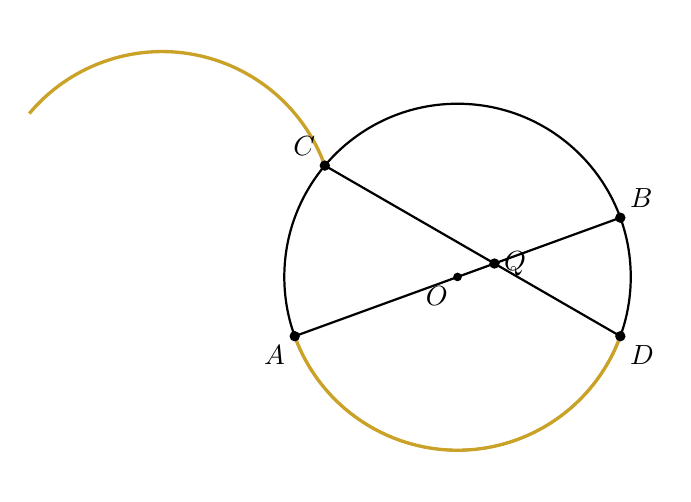
\begin{tikzpicture}[scale=1.1]
  % Lingkaran pusat O, jari-jari 2
  \coordinate (O) at (0,0);
  \draw[thick] (O) circle (2);
  \fill (O) circle (0.05) node[below left] {$O$};
  % Dua tali pengukur yang berpotongan di dalam lingkaran
  \coordinate (A) at (200:2);
  \coordinate (B) at (20:2);
  \coordinate (C) at (140:2);
  \coordinate (D) at (340:2);
  \coordinate (Q) at (intersection of A--B and C--D);
  \draw[thick] (A) -- (B);
  \draw[thick] (C) -- (D);
  \draw[very thick, color=goldenrod] (A) arc[start angle=200, end angle=340, radius=2];
  \draw[very thick, color=goldenrod] (C) arc[start angle=20, end angle=140, radius=2];
  \foreach \pt/\pos in {A/below left, B/above right, C/above left, D/below right, Q/right} {
    \fill (\pt) circle (0.06) node[\pos] {$\pt$};
  }
\end{tikzpicture}

\vspace{1em}
Sudut $\angle CQB$ puncaknya di $Q$ (di dalam lingkaran). Besarnya
$\angle CQB = \tfrac{1}{2}\left(\widehat{AB} + \widehat{CD}\right)$:
setengah jumlah busur yang dihadapinya.

\end{document}
